\documentclass[a4paper]{article}
\usepackage[utf8]{inputenc} % - Defines what coding LaTeX uses. Use this one.
\usepackage[swedish]{babel}
\usepackage{graphicx}
\graphicspath{ {./images/} }

\title{Sprint 4 - Slutrapport \\ 
\large{Laboration för D0018E - Databasteknik}}

\author{Josef Utbult \\
{\tt josutb-7@student.ltu.se}}
\date{\today}

\begin{document}

\maketitle
\newpage
\section{Introduktion}
Det här är en webbshop utvecklad för en laboration i kurset \textit{D0020E}. \textit{Musikdong}, som är webbshopens namn, säljer gitarrpedaler, fullt legala tjänster samt annat smått och gott. Nu är sidan färdig och sitter sidan uppe på IP-adressen http://130.240.200.51:5000. Servern är aktiv om man ber Josef att sätta på den, annars ligger den passiv.

\section{Executive summary}
\subsection{Sprint 1 - Josef}
Jag har jobbat med att sätta upp servern inför sprint 1. Vi använde den virtuella maskinen tillhandahållen av LUDD, där vi satt upp mySql som databas, en flask-applikation för att kommunicera med backenden samt Nginx för att komma åt sidan via vår statiska IP.

Jag har även experimenterat med att interagera med mySql, främst på min egen maskin för enkelhetens skull, men sett till så att allt är kompatibelt för att emigrera till den virtuella maskinen.

\subsection{Sprint 1 - Leo}
Jag har tillsammans med Josef tagit fram user stories samt gjort en enkel hemsida med html och css. 

\subsection{Sprint 2 - Josef}
Jag har byggt om databasen för att hantera produkter, kategorier och användare mm. Jag har även lagt till strukturen för orderhantering i databasen, i form av ett orders-table och ett orderItem-table. En grundläggande manager-sida har också lagts till.

\subsection{Sprint 3 - Josef}
Jag har byggt klart manager-sidan med möjlighet att lägga till produkter och kategorier, samt redigera användare, produkter och kategorier. Jag har fixat orderhanteringen och implementerat att priset låses efter att ordern läggs. Jag har även implementerat reviws. 

\subsection{Sprint 4 - Josef}
Jag har lagt till en sökbar i headern som söker på produktnamn.


\section{Userstories}
\subsection{Admin}
\begin{enumerate}
  \item Har alla rättigheter som manager.
  \item Kan ändra rättigheter för alla användare på sidan.
  \item Kan lägga till och radera
  %
  \begin{itemize}
    \item Kategorier
    \item Tagtyper
  \end{itemize}
\end{enumerate}
%
\subsection{Manager}
\begin{enumerate}
  \item Har alla rättigheter som en inloggad användare.
  \item Kan öppna en manager meny.
  \item Har tillgång till att redigera alla
  %
  \begin{itemize}
    \item Användare
    \item Produkter
    \item Kategorier 
    \item Tagtyper
    \item Reviews
    \item Carts
    \item Orders
  \end{itemize}
  %
  \item Kan få en lista med alla ordrar i manager-menyn, där man ser betalade ordrar samt hanterade ordrar separat.
  \item Kan lägga till och radera
  \begin{itemize}
  \item Användare
  \item Produkter
  \item Taggar
  \end{itemize}
\end{enumerate}
%
\subsection{Inloggad användare}
\begin{enumerate}
  \item Har alla rättigheter som en icke inloggad användare.
  \item Kan orientera sig mellan kategorier till produkter.
  \item Kan lägga produkter i sin kundvagn.
  \item Kan lägga en review på en produkt.
  \item Kan öppna sin kundvagn och se vad som ligger i.
  \item Kan lägga en order som senare hanteras av managers.
  \item Kan logga ut från sin användare.
\end{enumerate}
%
\subsection{Icke inloggad användare}
\begin{enumerate}
  \item Kan orientera sig mellan kategorier till produkter.
  \item Kan använda sökbaren för att söka på ett produktnamn.
  \item Kan logga in, eller skapa en användare.
\end{enumerate}
%
\section{Backlog}
%
\begin{figure}[h]
\caption{Backlog i slutet av projektet.}
\centering
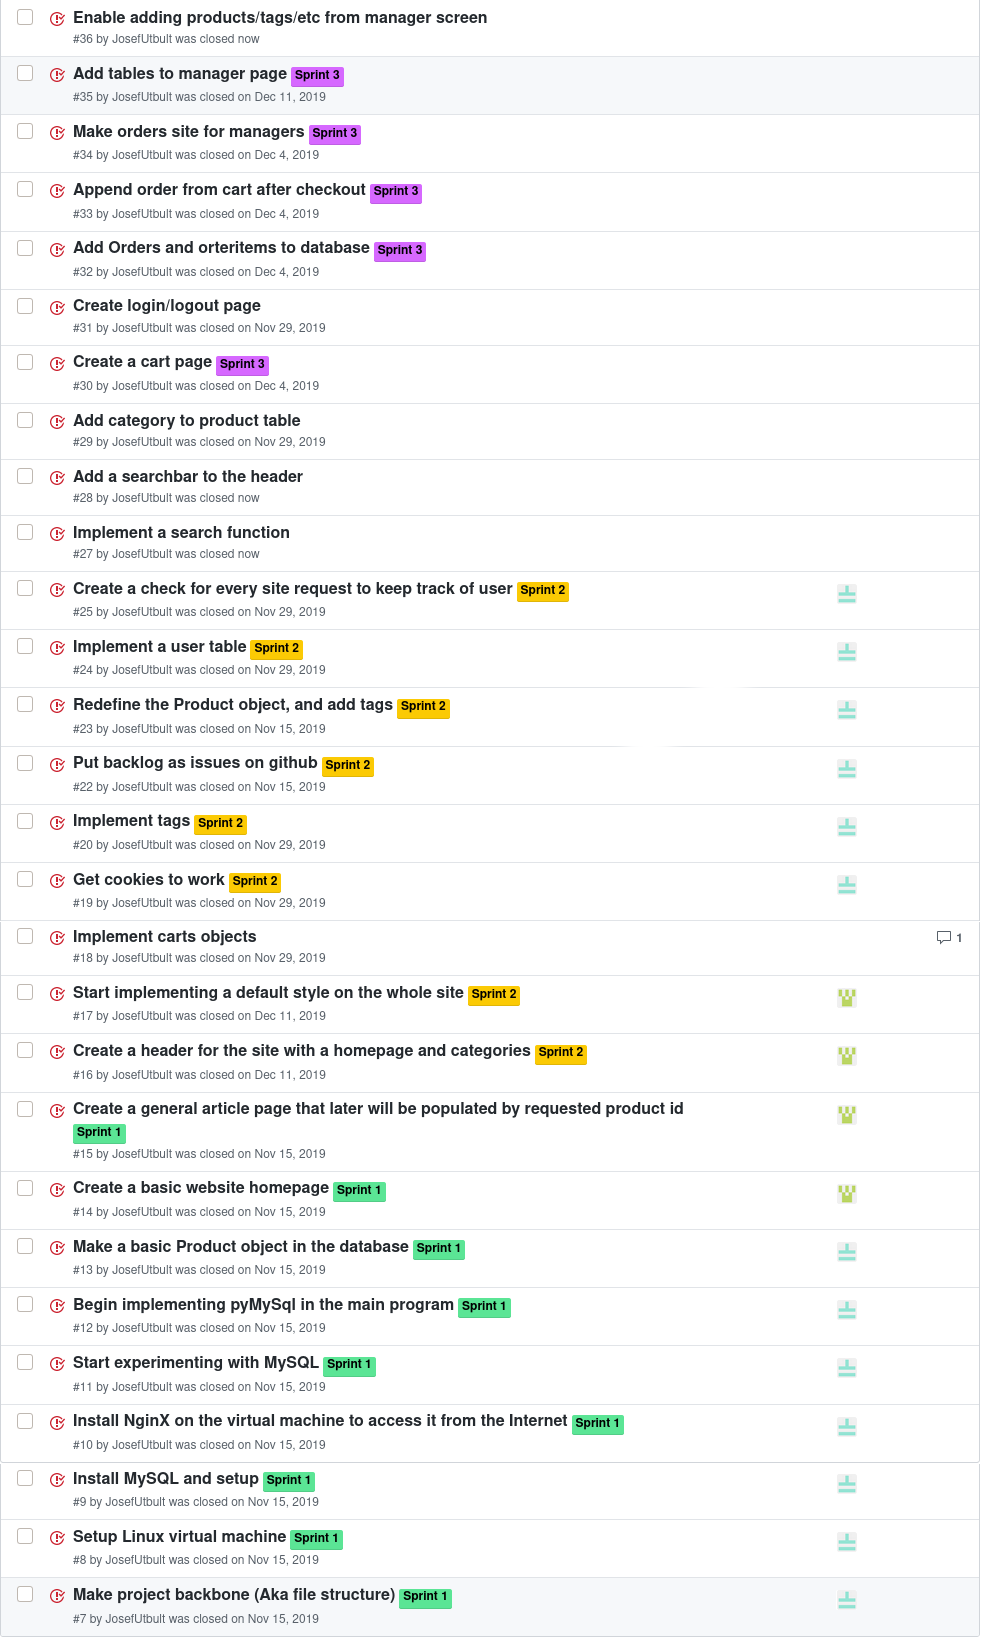
\includegraphics[width=0.5\textwidth]{Backlog.png}
\end{figure}
%
\end{document}

